\documentclass[11pt,border=5pt]{standalone}
\usepackage{fontspec}
\setmainfont{cmunrm.otf}[BoldFont=cmunbx.otf,ItalicFont=cmunti.otf,BoldItalicFont=cmunbi.otf]
\usepackage{amsmath}
\usepackage{unicode-math}
\setmathfont{NewCMMath-Regular.otf}
\usepackage{tikz}
\usetikzlibrary{arrows.meta,patterns,angles,quotes}
\begin{document}
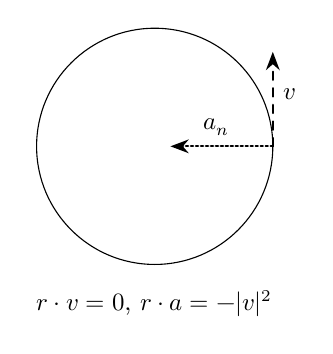
\begin{tikzpicture}[>=Stealth,font=\small,line cap=round,line join=round]
\draw (0,0) circle (1.5);
\draw[->,thick,dashed] (1.5,0) -- (1.5,1.2) node[pos=0.55,right] {$v$};
\draw[->,thick,densely dotted] (1.5,0) -- (0.2,0) node[pos=0.55,above] {$a_n$};
\node at (0,-2) {$r\cdot v=0$, $r\cdot a=-|v|^2$};

\end{tikzpicture}
\end{document}
